\documentclass{scrartcl} % scrartcl of scrreprt
% Include all project wide packages here.
\usepackage{fullpage}
\usepackage{polyglossia}
\setmainlanguage{dutch}
\usepackage{csquotes}
\usepackage{graphicx}
\usepackage{epstopdf}
\usepackage{pdfpages}
\usepackage{caption}
\usepackage[list=true]{subcaption}
\usepackage{float}
%\usepackage{mathtools}
\usepackage{standalone}
\usepackage{import}
\usepackage{tocloft}
\usepackage{wrapfig}
\usepackage{authblk}
\usepackage{array}
\usepackage{booktabs}
\usepackage[toc,page,title,titletoc]{appendix}
\usepackage{xunicode}
\usepackage{amsmath}
\usepackage{fontspec}
\usepackage{unicode-math}
\usepackage[
    backend=bibtexu,
	texencoding=utf8,
bibencoding=utf8,
    style=ieee,
    sortlocale=nl_NL,
    language=auto
]{biblatex}
\usepackage{listings}
\newcommand{\includecode}[3][c]{\lstinputlisting[caption=#2, escapechar=, style=#1]{#3}}
\newcommand{\superscript}[1]{\ensuremath{^{\textrm{#1}}}}
\newcommand{\subscript}[1]{\ensuremath{_{\textrm{#1}}}}


\newcommand{\chapternumber}{\thechapter}
\renewcommand{\appendixname}{Bijlage}
\renewcommand{\appendixtocname}{Bijlagen}
\renewcommand{\appendixpagename}{Bijlagen}

\usepackage[hidelinks]{hyperref} %<--------ALTIJD ALS LAATSTE

\renewcommand{\familydefault}{\sfdefault}

\setmainfont[Ligatures=TeX]{Myriad Pro}
\setmathfont{Asana Math}
\setmonofont{Lucida Console}

\usepackage{titlesec, blindtext, color}
\definecolor{gray75}{gray}{0.75}
\newcommand{\hsp}{\hspace{20pt}}
\titleformat{\chapter}[hang]{\Huge\bfseries}{\chapternumber\hsp\textcolor{gray75}{|}\hsp}{0pt}{\Huge\bfseries}
\renewcommand{\familydefault}{\sfdefault}
\renewcommand{\arraystretch}{1.2}
\setlength\parindent{0pt}

%For code listings
\definecolor{black}{rgb}{0,0,0}
\definecolor{browntags}{rgb}{0.65,0.1,0.1}
\definecolor{bluestrings}{rgb}{0,0,1}
\definecolor{graycomments}{rgb}{0.4,0.4,0.4}
\definecolor{redkeywords}{rgb}{1,0,0}
\definecolor{bluekeywords}{rgb}{0.13,0.13,0.8}
\definecolor{greencomments}{rgb}{0,0.5,0}
\definecolor{redstrings}{rgb}{0.9,0,0}
\definecolor{purpleidentifiers}{rgb}{0.01,0,0.01}


\lstdefinestyle{csharp}{
language=[Sharp]C,
showspaces=false,
showtabs=false,
breaklines=true,
showstringspaces=false,
breakatwhitespace=true,
escapeinside={(*@}{@*)},
columns=fullflexible,
commentstyle=\color{greencomments},
keywordstyle=\color{bluekeywords}\bfseries,
stringstyle=\color{redstrings},
identifierstyle=\color{purpleidentifiers},
basicstyle=\ttfamily\small}

\lstdefinestyle{c}{
language=C,
showspaces=false,
showtabs=false,
breaklines=true,
showstringspaces=false,
breakatwhitespace=true,
escapeinside={(*@}{@*)},
columns=fullflexible,
commentstyle=\color{greencomments},
keywordstyle=\color{bluekeywords}\bfseries,
stringstyle=\color{bluestrings},
identifierstyle=\color{purpleidentifiers}
}

\lstdefinestyle{vhdl}{
language=VHDL,
showspaces=false,
showtabs=false,
breaklines=true,
showstringspaces=false,
breakatwhitespace=true,
escapeinside={(*@}{@*)},
columns=fullflexible,
commentstyle=\color{greencomments},
keywordstyle=\color{bluekeywords}\bfseries,
stringstyle=\color{redstrings},
identifierstyle=\color{purpleidentifiers}
}

\lstdefinestyle{xaml}{
language=XML,
showspaces=false,
showtabs=false,
breaklines=true,
showstringspaces=false,
breakatwhitespace=true,
escapeinside={(*@}{@*)},
columns=fullflexible,
commentstyle=\color{greencomments},
keywordstyle=\color{redkeywords},
stringstyle=\color{bluestrings},
tagstyle=\color{browntags},
morestring=[b]",
  morecomment=[s]{<?}{?>},
  morekeywords={xmlns,version,typex:AsyncRecords,x:Arguments,x:Boolean,x:Byte,x:Char,x:Class,x:ClassAttributes,x:ClassModifier,x:Code,x:ConnectionId,x:Decimal,x:Double,x:FactoryMethod,x:FieldModifier,x:Int16,x:Int32,x:Int64,x:Key,x:Members,x:Name,x:Object,x:Property,x:Shared,x:Single,x:String,x:Subclass,x:SynchronousMode,x:TimeSpan,x:TypeArguments,x:Uid,x:Uri,x:XData,Grid.Column,Grid.ColumnSpan,Click,ClipToBounds,Content,DropDownOpened,FontSize,Foreground,Header,Height,HorizontalAlignment,HorizontalContentAlignment,IsCancel,IsDefault,IsEnabled,IsSelected,Margin,MinHeight,MinWidth,Padding,SnapsToDevicePixels,Target,TextWrapping,Title,VerticalAlignment,VerticalContentAlignment,Width,WindowStartupLocation,Binding,Mode,OneWay,xmlns:x}
}

%defaults
\lstset{
basicstyle=\ttfamily\small,
extendedchars=false,
numbers=left,
numberstyle=\ttfamily\tiny,
stepnumber=1,
tabsize=4,
numbersep=5pt
}
\addbibresource{../../library/bibliography.bib}

\author{}
\title{EPO3: Eindrapport - Ontwerp}

\begin{document}
\chapter{Ontwerp}
\label{ch:ontwerp}

Ons GPU is ingedeeld volgens Figure ~\ref{fig:Blokschema GPU}.

\begin{figure}[H]
\centering
	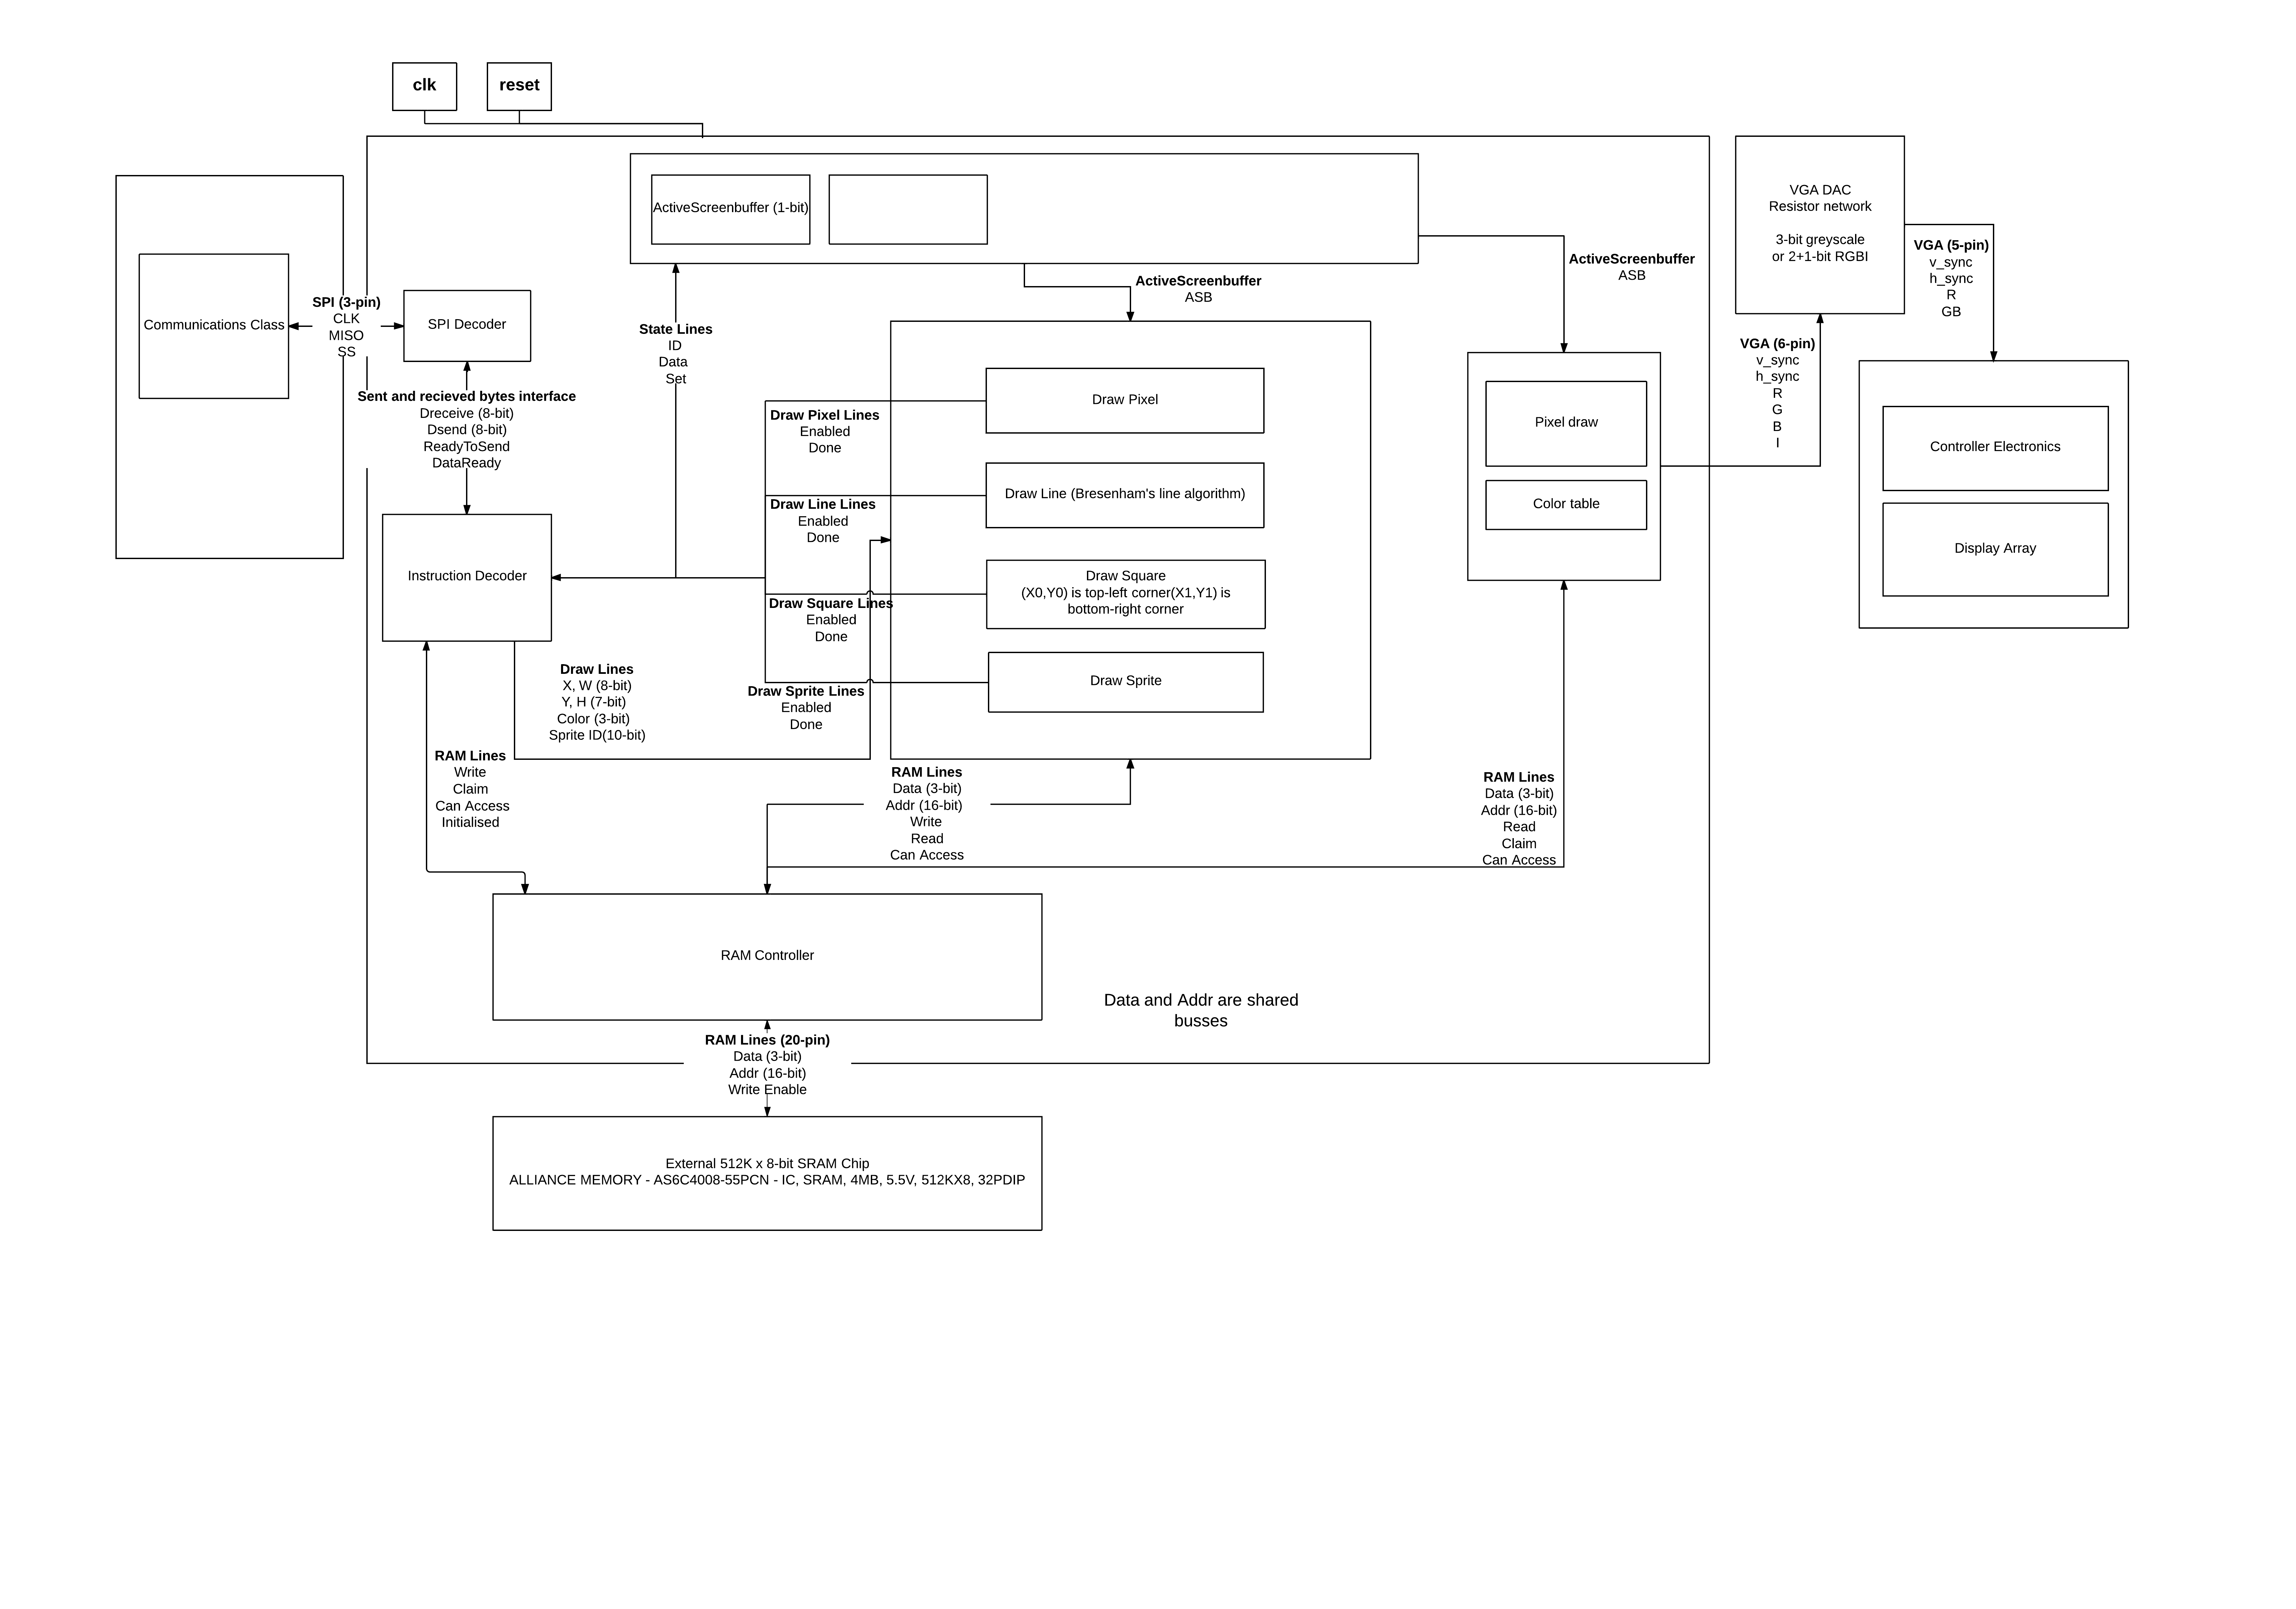
\includegraphics[width=\linewidth, angle=90]{resource/systeemdrawing-v2.png}
	\caption{Blokschema GPU}
	\label{fig:Blokschema GPU}
\end{figure}

\section{Parameters}
In Tabel \ref{tab:spec-params} staat een overzicht van de gebruikte parameters en generics.

\begin{table}[H]
\centering
\caption{De gebruikte parameters en generics}
\label{tab:spec-params}
\begin{tabular}{l l l l l}
	\hline\hline
 	 & Naam & Type & Waarde & Omschrijving\\
 	\hline
	%GLOBAL
	pkg & InstrSize & integer & 3 & De grootte van een instructie\\ 
	pkg & MaxNumPackets & integer & 3 & Maximaal aantal pakketjes in één instructie\\ 
	pkg & SizeSpriteID & integer & 10 & Het aantal bits voor het SpriteID \\
	pkg & SizeSpriteCounter & integer & 6 & Het aantal bits voor de sprite counter\\
	pkg & SizeTimeoutCounter & integer & 7 & Het aantal bits voor de timout counter\\
	pkg & NumDrawModules & integer & 5 & Aantal Draw modules\\ 
	pkg & SizeX & integer & 8 & Het aantal bits voor de X coordinaat\\
	pkg & SizeY & integer & 7 & Het aantal bits voor de Y coordinaat\\
	pkg & NumStateReg & integer & 1 & Aantal globale state registers\\
	pkg & SizeRAMData & integer & 3 & Aantal bits per woord in het RAM\\
	pkg & SizeRAMAddr & integer & 16 & Aantal adresbits voor het RAM\\
	pkg & SizeColor & integer & 3 & Aantal bits kleur\\
	pkg & SizeSPIData & integer & 8 & Aantal bits van de SPI pakketjes\\
	pkg & ResolutionX & integer & 160 & Horizontale resolutie \\
	pkg & ResolutionY & integer & 120 & Verticale resolutie \\
	%VGA
	vga & h\_pulse & integer & 24 & Aantal klokpulsen voor de horizontale syncpuls\\ 
	vga & h\_bp & integer & 12 & Aantal klokpulsen voor de horizontale “backporch” \\ 
	vga & h\_pixels & integer & 160 & Aantal klokpulsen voor de horizontale pixels \\ 
	vga & h\_fp & integer & 4 & Aantal klokpulsen voor de horizontale “fontporch” \\ 
	vga & h\_pol & std\_logic & ‘0’ & De polariteit van de horizontale syncpuls\\ 
	vga & v\_pulse & integer & 2 & Aantal rijen voor de verticale syncpuls\\ 
	vga & v\_bp & integer & 33 & Aantal rijen voor de verticale “backporch” \\ 
	vga & v\_pixels & integer & 480 & Aantal rijen voor de verticale pixels\\ 
	vga & v\_fp & integer & 10 & Aantal rijen voor de verticale “fontporch” \\ 
	vga & v\_pol & std\_logic & ‘0’ & De polariteit van de verticale syncpuls\\ 
	%SPI
	spi & c & integer & 4 & Het aantal bits van de counter in de SPI module\\
  	\hline
\end{tabular}
\end{table}

\section{SPI Controller}
Voor de communicatie tussen de AVR en onze GPU hebben we een SPI decoder nodig.
De ingang SS staat voor slave select, deze wordt normaal gebruikt voor het geval dat je meerdere slave chips hebt, aangezien dit bij ons niet het geval is zal dit signaal altijd hoog zijn.
De in- en uitgangen zijn gespecificeerd in Tabel \ref{tab:spec-spi}.

\begin{table}[H]
\centering
\caption{Specificaties van de SPI Controller (spi)}
\label{tab:spec-spi}
\begin{tabular}{c c c}
	\hline\hline
 	Naam & Modus & Type\\
 	\hline
	clk & in & std\_logic \\
	reset & in & std\_logic \\
	spi\_clk & in & std\_logic \\
	spi\_ss & in & std\_logic \\
	spi\_mosi & in & std\_logic \\
	spi\_data\_available & out & std\_logic \\
	spi\_data\_rx & out & std\_logic\_vector(SizeSPIData-1 downto 0) \\
  	\hline
\end{tabular}
\end{table}

\section{Instruction Decoder}
De instructiedecoder is er om de door de AVR geleverde data te vertalen naar data (een instructie), waar de draw-module mee over weg kan.
De decoder leest van SPI-interface een byte (SPIDataRxd), wanneer de SPI-interface aangeeft dat deze klaar staat (SPIDataAvailable).
Deze byte wordt vervolgens afhankelijk van een interne counter vertaald naar een instructie, kleur of coördinaat.
Wanneer de decoder met zijn ingebouwde counter bepaalt dat de instructiedata (één of meer bytes) geheel ontvangen is, wordt de bijbehorende actie ondernomen.
Dit houdt in dat de gewenste draw-module wordt geactiveerd (met het signaal en), of het screen buffer wordt omgewisseld (reg\_id, reg\_value, reg\_set).
Het actieve screen buffer wordt bijgehouden in een globaal register.
Dit alles gebeurt uiteraard geheel synchroon en uitgangsdata blijft beschikbaar tot de volgende instructie door middel van flip-flops.
De in- en uitgangen zijn gespecificeerd in Tabel \ref{tab:spec-decoder}.

\begin{table}[H]
\centering
\caption{Specificaties van de Insctructie Decoder (decoder)}
\label{tab:spec-decoder}
\begin{tabular}{c c c}
	\hline\hline
 	Naam & Modus & Type\\
 	\hline
	clk & in & std\_logic \\
	reset & in & std\_logic \\	
	spi\_data\_rx & out & std\_logic\_vector(SizeSPIData-1 downto 0) \\
	spi\_data\_available & in & std\_logic \\
	x &  buffer & std\_logic\_vector(SizeX-1 downto 0) \\
	w &  buffer & std\_logic\_vector(SizeX-1 downto 0) \\
	y &  buffer & std\_logic\_vector(SizeY-1 downto 0) \\
	h &  buffer & std\_logic\_vector(SizeY-1 downto 0) \\
	color &  buffer & std\_logic\_vector(SizeColor-1 downto 0) \\
	en & buffer & std\_logic\_vector(NumDrawModules-1 downto 0)\\
	decoder\_can\_access & in & std\_logic \\
	decoder\_claim & out & std\_logic \\
	is\_init & out & std\_logic \\
  	\hline
\end{tabular}
\end{table}

\section{Draw Module}
In dit blok worden de instructie omgezet naar pixels, rechthoeken en lijnen, die met kleur gevuld kunnen worden.
Dit blok krijgt de informatie binnen van de instructiedecoder, deze geeft aan welke module er gebruikt moet worden met de bijbehorende data (x, y, etc.), ook is er een input die het huidige screen buffer aanduidt (asb).
De draw module schijft naar het niet-actieve screenbuffer.
Verder bevat de module de benodigde signals om naar het RAM te schrijven (ramaddr en ramdata) en om te bepalen of er naar het RAM geschreven kan worden op een bepaald moment (draw\_write, draw\_read, draw\_can\_access).

De in- en uitgangen zijn gespecificeerd in Tabel \ref{tab:spec-draw}.

\begin{table}[H]
\centering
\caption{Specificaties van de Draw Module (draw)}
\label{tab:spec-draw}
\begin{tabular}{c c c}
	\hline\hline
 	Naam & Modus & Type\\
 	\hline	
	 clk & in & std\_logic \\
	 reset & in & std\_logic \\
	id & in & std\_logic\_vector(SizeSpriteID-1 downto 0) \\
	 x & in & std\_logic\_vector(SizeX-1 downto 0) \\ 
	 w & in & std\_logic\_vector(SizeX-1 downto 0) \\
	 y & in & std\_logic\_vector(SizeY-1 downto 0) \\
	 h & in & std\_logic\_vector(SizeY-1 downto 0) \\ 
	 color & in & std\_logic\_vector(SizeColor-1 downto 0) \\ 
	 en & in & std\_logic\_vector(NumDrawModules-1 downto 0) \\ 
	 draw\_ready & out & std\_logic \\
	 asb & in & std\_logic \\ 
	 draw\_write & out & std\_logic \\
	 draw\_read & out & std\_logic \\
	 draw\_can\_access & in & std\_logic \\
	 ramaddr & out & std\_logic\_vector(SizeRAMAddr-1 downto 0) \\
	 ramdata & out & std\_logic\_vector(SizeRAMData-1 downto 0) \\
  	\hline
\end{tabular}
\end{table}

\subsection {Fill}
De Fill-module verandert in één instructie het hele beeldscherm naar een gegeven kleur.

\begin{table}[H]
\centering
\caption{Specificaties van de Fill Draw Module}
\label{tab:spec-fill-draw}
\begin{tabular}{c c c}
	\hline\hline
 	Naam & Modus & Type\\
 	\hline	
	clk & in & std\_logic \\
	reset & in & std\_logic \\
	enable& in & std\_logic \\
	color & in & std\_logic\_vector(SizeColor-1 downto 0) \\
	asb & in & std\_logic \\
	done & out & std\_logic \\
	ramaddr &out & std\_logic\_vector(SizeRAMAddr-1 downto 0) \\
	ramdata &out & std\_logic\_vector(SizeRAMData-1 downto 0) \\
	draw\_write &out & std\_logic \\
	draw\_can\_access & in & std\_logic \\
  	\hline
\end{tabular}
\end{table}

\subsection {Pixel}
Door deze module worden aparte pixels getekend, hiervoor zijn de x- en y-coördinaten en de kleur van de pixel nodig.

\begin{table}[H]
\centering
\caption{Specificaties van de Pixel Draw Module}
\label{tab:spec-pixel-draw}
\begin{tabular}{c c c}
	\hline\hline
 	Naam & Modus & Type\\
 	\hline	
	clk & in & std\_logic \\
	reset & in & std\_logic \\
	enable& in & std\_logic \\
	color & in & std\_logic\_vector(SizeColor-1 downto 0) \\
	x & in & std\_logic\_vector(SizeX-1 downto 0) \\
	y & in & std\_logic\_vector(SizeY-1 downto 0) \\
	asb & in & std\_logic \\
	done & out & std\_logic \\
	ramaddr &out & std\_logic\_vector(SizeRAMAddr-1 downto 0) \\
	ramdata &out & std\_logic\_vector(SizeRAMData-1 downto 0) \\
	draw\_write &out & std\_logic \\
	draw\_can\_access & in & std\_logic \\
  	\hline
\end{tabular}
\end{table}

\subsection {Line}
Deze module kan lijnen tekenen aan de hand van 2 coördinaten. Met deze coördinaten wordt er gerekend aan de hand van Bresenham's lijn algoritme welke pixels nodig zijn om de 2 coördinaten met een lijn te verbinden.

\begin{table}[H]
\centering
\caption{Specificaties van de Line Draw Module}
\label{tab:spec-line-draw}
\begin{tabular}{c c c}
	\hline\hline
 	Naam & Modus & Type\\
 	\hline	
	clk & in & std\_logic \\
	reset & in & std\_logic \\
	enable& in & std\_logic \\
	color & in & std\_logic\_vector(SizeColor-1 downto 0) \\
	x0 & in & std\_logic\_vector(SizeX-1 downto 0) \\
	y0 & in & std\_logic\_vector(SizeY-1 downto 0) \\
	x1 & in & std\_logic\_vector(SizeX-1 downto 0) \\
	y1 & in & std\_logic\_vector(SizeY-1 downto 0) \\
	asb & in & std\_logic \\
	done & out & std\_logic \\
	ramaddr &out & std\_logic\_vector(SizeRAMAddr-1 downto 0) \\
	ramdata &out & std\_logic\_vector(SizeRAMData-1 downto 0) \\
	draw\_write &out & std\_logic \\
	draw\_can\_access & in & std\_logic \\
  	\hline
\end{tabular}
\end{table}

\subsection {Rectangle}
In deze module wordt een rechthoek getekend met de x- en y-coördinaten van de eerste pixel links boven en de gegeven afmetingen. De rechthoek kan ook met kleur ingevuld worden. 

\begin{table}[H]
\centering
\caption{Specificaties van de Rectangle Draw Module}
\label{tab:spec-rect-draw}
\begin{tabular}{c c c}
	\hline\hline
 	Naam & Modus & Type\\
 	\hline	
	clk & in & std\_logic \\
	reset & in & std\_logic \\
	enable& in & std\_logic \\
	enablef& in & std\_logic \\
	color & in & std\_logic\_vector(SizeColor-1 downto 0) \\
	x & in & std\_logic\_vector(SizeX-1 downto 0) \\
	y & in & std\_logic\_vector(SizeY-1 downto 0) \\
	w & in & std\_logic\_vector(SizeX-1 downto 0) \\
	h & in & std\_logic\_vector(SizeY-1 downto 0) \\
	asb & in & std\_logic \\
	done & out & std\_logic \\
	ramaddr &out & std\_logic\_vector(SizeRAMAddr-1 downto 0) \\
	ramdata &out & std\_logic\_vector(SizeRAMData-1 downto 0) \\
	draw\_write &out & std\_logic \\
	draw\_can\_access & in & std\_logic \\
  	\hline
\end{tabular}
\end{table}

\subsection {Sprite}
In deze module wordt een sprite uitgelezen/ingeschreven vanuit het RAM en getekend op het scherm aan de hand van de x- en y- coördinaten van de eerste pixel links boven en de gegeven afmetingen van de sprite.
\begin{table}[H]
\centering
\caption{Specificaties van de Sprite Draw Module}
\label{tab:spec-sprite-draw}
\begin{tabular}{c c c}
	\hline\hline
 	Naam & Modus & Type\\
 	\hline	
	clk & in & std\_logic \\
	reset & in & std\_logic \\
	enable& in & std\_logic \\
	id & in & std\_logic\_vector(SizeSpriteID-1 downto 0) \\
	color & in & std\_logic\_vector(SizeColor-1 downto 0) \\
	x & in & std\_logic\_vector(SizeX-1 downto 0) \\
	y & in & std\_logic\_vector(SizeY-1 downto 0) \\
	w & in & std\_logic\_vector(SizeX-1 downto 0) \\
	l & in & std\_logic\_vector(SizeSpriteCounter-1 downto 0) \\
	asb & in & std\_logic \\
	done & out & std\_logic \\
	ramaddr &out & std\_logic\_vector(SizeRAMAddr-1 downto 0) \\
	ramdata &out & std\_logic\_vector(SizeRAMData-1 downto 0) \\
	draw\_write &out & std\_logic \\
	draw\_read&out & std\_logic \\
	draw\_can\_access & in & std\_logic \\
  	\hline
\end{tabular}
\end{table}

\section{RAM Controller}
Omdat we een externe RAM gebruiken voor onze screenbuffers is het nodig om hiervoor communicatie op te stellen, zodat er in het juiste gedeelte van de RAM geschreven en gelezen wordt en dat dit niet tegelijkertijd gebeurd, omdat het RAM dat niet aankan. We hebben voor een externe RAM gekozen omdat er geen RAM geheugen groot genoeg gemaakt kon worden met de benodigde transistoren om bijvoorbeeld de screenbuffers te renderen. De RAM controller stuurt naar het draw-blok een signaal write als het mag gaan schrijven in het RAM geheugen, de RAM controller krijgt dan de kleur en het adress binnen van het draw-blok. Als de VGA controller mag gaan lezen krijgt het een signaal read binnen van de RAM controller dan zal er weer data naar de VGA controller verstuurd worden, kleur en adres.

\begin{table}[H]
\centering
\caption{Specificaties van de RAM Controller (ramcontroller)}
\label{tab:spec-ramcontroller}
\begin{tabular}{c c c}
	\hline\hline
 	Naam & Modus & Type\\
 	\hline	
	write\_enable & out & std\_logic\\
	vga\_claim & in & std\_logic\\
	decoder\_claim & in & std\_logic\\
	is\_init & in & std\_logic\\
	decoder\_write & in & std\_logic\\
	draw\_write & in & std\_logic\\
	draw\_read & in & std\_logic\\
	vga\_read & in & std\_logic\\
	draw\_can\_access & out & std\_logic\\
	decoder\_can\_access & out & std\_logic\\
	vga\_can\_access & out & std\_logic\\
  	\hline
\end{tabular}
\end{table}

\section{VGA Controller}
De VGA-controller leest het actieve screen buffer uit het RAM en zet de gelezen data om in beelduitvoer.

\begin{table}[H]
\centering
\caption{Specificaties van de VGA Controller (vgacontroller)}
\label{tab:spec-vgacontroller}
\begin{tabular}{c c c}
	\hline\hline
 	Naam & Modus & Type\\
 	\hline	
	clk & in & std\_logic \\ 
	reset\_n & in & std\_logic \\ 
	vgahsync & out & std\_logic \\ 
	vgavsync & out & std\_logic \\ 
	vgacolor & out & std\_logic\_vector(SizeColor-1 downto 0) \\
	vga\_claim & out & std\_logic \\ 
	ramaddr & out & std\_logic\_vector(SizeRAMAddr-1 downto 0) \\
	ramdata & in & std\_logic\_vector(SizeRAMData-1 downto 0) \\ 
	vga\_read & out & std\_logic \\
	vga\_can\_access & in & std\_logic \\
	asb & in & std\_logic \\
  	\hline
\end{tabular}
\end{table}

\end{document}
